\chapter{Grenzen kontextfreier Sprachen} 
In diesem Kapitel diskutieren wir die Grenzen kontextfreier Sprachen und leiten dazu dass
sogenannte ``\emph{gro{\ss}e Pumping-Lemma}'' her, mit dessen Hilfe wir beispielsweise zeigen
k\"onnen, dass die Sprache $L_{\mbox{\scriptsize \textsl{square}}}$, die durch
\\[0.2cm]
\hspace*{1.3cm} $L_{\mbox{\scriptsize \textsl{square}}} = \bigl\{ ww \mid w \in \Sigma^*\bigr\}$
\\[0.2cm]
definiert wird, f\"ur das Alphabet $\Sigma =\{\texttt{a}, \texttt{b}\}$ keine kontextfreie Sprache ist.


\section{Die verallgemeinerte Chomsky-Normalform}
In diesem Abschnitt zeigen wir, wie eine kontextfreie Sprache in die \emph{verallgemeinerte Chomsky-Normal\-form}
(vCNF) \"uberf\"uhrt werden kann.  Die \"Uberf\"uhrung einer Sprache in verallgemeinerte
Chomsky-Normalform erfolgt in mehreren Schritten.
\begin{enumerate}
\item Zun\"achst beseitigen wir \emph{nutzlose Symbole}.

      Ist $G = \langle V, T, R, S \rangle$ eine Grammatik, so nennen wir eine syntaktische Variable $A \in V$
      \emph{n\"utzlich}, wenn es einen String $w \in T^*$ sowie Strings $\alpha,\beta \in (V \cup T)^*$ gibt, 
      so dass 
      \\[0.2cm]
      \hspace*{1.3cm}
      $S \Rightarrow^* \alpha A \beta \Rightarrow^* w$
      \\[0.2cm]
      gilt.  Eine syntaktische Variable ist also genau dann n\"utzlich, wenn diese Variable in der Herleitung
      eines Wortes $w \in L(G)$ verwendet werden kann.

      Ein Terminal $t$ ist \emph{n\"utzlich}, wenn es W\"orter $w_1, w_2 \in T^*$ gibt, so dass
      \\[0.2cm]
      \hspace*{1.3cm}
      $S \Rightarrow^* w_1 t w_2$
      \\[0.2cm]
      gilt.  Ein Terminal $t$ ist also genau dann n\"utzlich, wenn es in einem Wort der Sprache $L(G)$
      auftritt.  Variablen und Terminale, die nicht n\"utzlich sind, bezeichnen wir als
      \emph{nutzlose Symbole}.
\item Anschlie{\ss}end zeigen wir, dass alle \emph{$\varepsilon$-Regeln} aus der Grammatik eliminiert werden k\"onnen.
      Dabei bezeichnen wir eine Grammatik-Regel der Form
      \\[0.2cm]
      \hspace*{1.3cm}
      $A \rightarrow \varepsilon$
      \\[0.2cm]
      als eine \emph{$\varepsilon$-Regel}.
\item Schlie{\ss}lich zeigen wir, wie alle Grammatik-Regeln der Form 
      \\[0.2cm]
      \hspace*{1.3cm}
      $A \rightarrow B$
      \\[0.2cm]
      mit $A,B \in V$ eliminiert werden k\"onnen.  Solche Grammatik-Regeln werden als
      \emph{Unit-Regeln} bezeichnet.
\end{enumerate}

\subsection{Beseitigung nutzloser Symbole}
Die Erkennung nutzloser Symbole ist eine \"Uberpr\"ufung, die in manchen Parser-Generatoren
(beispielsweise in \textsl{Bison}\footnote{
\textsl{Bison} ist ein Parser-Generator f\"ur die Sprache \texttt{C}.}) 
eingebaut ist, weil das Auftreten nutzloser Symbole oft
einen Hinweis darauf gibt, dass die Grammatik nicht die Sprache beschreibt, die intendiert ist.  
Insofern ist die jetzt vorgestellte Technik auch von praktischem Interesse.
Wir beginnen mit zwei Definitionen.

\begin{Definition}[erzeugende Variable] \lb
Eine syntaktische Variable $A \in V$ einer Grammatik $G = \langle V, T, R, S \rangle$ 
ist eine \emph{erzeugende} Variable, wenn es ein Wort $w \in T^*$ gibt, so dass
\\[0.2cm]
\hspace*{1.3cm}
$A \Rightarrow^* w$
\\[0.2cm]
gilt, aus einer erzeugende Variable l\"asst sich also immer mindestens ein Wort aus $T^*$ herleiten. 
Die Notation $A \Rightarrow^* w$ dr\"uckt aus, dass das Wort $w$ aus der Variablen $A$ in endlich vielen
Schritten abgeleitet werden kann.
\qed 
\end{Definition}

\noindent
Offenbar ist eine syntaktische Variable, die nicht erzeugend ist, nutzlos.  Die Menge aller
erzeugenden Variablen einer Grammatik $G$  kann mit Hilfe der folgenden induktiven Definition
gefunden werden.
\begin{enumerate}
\item Enth\"alt die Grammatik $G = \langle V, T, R, S \rangle$ eine Regel der Form
      \\[0.2cm]
      \hspace*{1.3cm}
       $A \rightarrow w$ \quad mit $w \in T^*$, 
      \\[0.2cm]
      so ist die Variable $A$ offenbar erzeugend.
\item Enth\"alt die Grammatik $G = \langle V, T, R, S \rangle$ eine Regel der Form
      \\[0.2cm]
      \hspace*{1.3cm}
       $A \rightarrow \alpha$ 
      \\[0.2cm]
      und sind alle syntaktischen Variablen, die in dem Wort $\alpha$ auftreten, bereits
      als erzeugende Variablen 
      erkannt, so ist auch die syntaktische Variable $A$ erzeugend.
\end{enumerate}

\example
Es sei $G = \langle \{S, A, B, C\}, \{ \texttt{x} \}, R, S \rangle$ und die Menge der Regeln $R$
sei wie folgt gegeben:
\begin{eqnarray*}
  S & \rightarrow & A B C \mid A,           \\
  A & \rightarrow & A A \mid \texttt{x},    \\
  B & \rightarrow & A C,                    \\
  C & \rightarrow & B A.                    
\end{eqnarray*}
Aufgrund der Regel
\\[0.2cm]
\hspace*{1.3cm}
$A \rightarrow \texttt{x}$
\\[0.2cm]
ist zun\"achst $A$ erzeugend.  Aufgrund der Regel
\\[0.2cm]
\hspace*{1.3cm}
$S \rightarrow A$
\\[0.2cm]
ist dann auch $S$ erzeugend.  Die Variablen $B$ und $C$ sind hingegen nicht erzeugend und damit sicher
nutzlos.  \qed
\vspace*{0.2cm}


\noindent
Ist $G = \langle V, T, R, S \rangle$ eine Grammatik und ist $E$ die Menge der erzeugenden Variablen,
so k\"onnen wir alle Variablen, die nicht erzeugend sind, einfach weglassen.  Zus\"atzlich m\"ussen wir
nat\"urlich auch die Regeln weglassen, in denen Variablen auftreten, die nicht erzeugend sind.  Dabei
\"andert sich die von der Grammatik $G$ erzeugte Sprache offenbar nicht.
\pagebreak

Eine Variable kann gleichzeitig erzeugend und trotzdem nutzlos sein.  Als einfaches
Beispiel betrachten wir die Grammatik  $G = \langle \{S, A, B \}, \{ \texttt{x}, \texttt{y} \}, R, S \rangle$, deren Regeln durch
\begin{eqnarray*}
  S & \rightarrow & A \texttt{y},           \\
  A & \rightarrow & A A \mid \texttt{x} \quad \mbox{und}    \\
  B & \rightarrow & A \texttt{y} 
\end{eqnarray*}
gegeben sind.  Die erzeugenden Variable sind in diesem Falle $A$, $B$ und $S$.  Die Variable
$B$ ist trotzdem nutzlos, denn von $S$ aus ist diese Variable gar nicht \emph{erreichbar}.
Formal definieren wir f\"ur eine Grammatik $G = \langle V, T, R, S \rangle$ eine syntaktische Variable $X$ als
\emph{erreichbar}, wenn es W\"orter $\alpha, \beta \in (V \cup T)^*$ gibt, so dass 
\\[0.2cm]
\hspace*{1.3cm}
$S \Rightarrow^* \alpha X \beta$
\\[0.2cm]
gilt. F\"ur eine gegebene Grammatik $G$  l\"asst sich die Menge der Variablen, die erreichbar
sind, mit dem folgenden 
induktiven Algorithmus berechnen.
\begin{enumerate}
\item Das Start-Symbol $S$ ist erreichbar.
\item Enth\"alt die Grammatik $G$ eine Regel der Form
      \\[0.2cm]
      \hspace*{1.3cm}
      $X \rightarrow \alpha$
      \\[0.2cm]
      und ist $X$ erreichbar, so sind auch alle Variablen, die in $\alpha$ auftreten, erreichbar.
\end{enumerate}
Offenbar sind Variablen, die nicht erreichbar sind, nutzlos und wir k\"onnen diese Variablen, sowie alle
Regeln, in denen diese Variablen auftreten, weglassen, ohne dass sich dabei die Sprache \"andert.
Damit haben wir jetzt ein Verfahren, um aus einer Grammatik alle nutzlosen Variablen zu entfernen.
\begin{enumerate}
\item Zun\"achst entfernen wir alle Variablen, die nicht erzeugend sind.
\item Anschlie{\ss}end entfernen wir alle Variablen, die nicht erreichbar sind.
\end{enumerate}
Es ist wichtig zu verstehen, dass die Reihenfolge der obigen Regeln nicht umgedreht werden darf.
Dazu betrachten wir die Grammatik  $G = \langle \{S, A, B, C\}, \{ \texttt{x}, \texttt{y} \}, R, S \rangle$, deren Regeln durch
\begin{eqnarray*}
  S & \rightarrow & B C \mid A,             \\
  A & \rightarrow & A A \mid \texttt{x},    \\
  B & \rightarrow & \texttt{y} \hspace*{1.3cm} \mbox{und} \\
  C & \rightarrow & C C 
\end{eqnarray*}
gegeben sind.  Die beiden Regeln
\\[0.2cm]
\hspace*{1.3cm}
$S \rightarrow BC$ \quad und \quad $S \rightarrow A$
\\[0.2cm]
zeigen, dass alle Variablen erreichbar sind.  Weiter sehen wir, dass die Variablen $A$, $B$ und $S$
erzeugend sind, denn es gilt
\\[0.2cm]
\hspace*{1.3cm}
$A \Rightarrow^* \texttt{x}$, \quad
$S \Rightarrow^* \texttt{x}$  \quad und \quad
$B \Rightarrow^* \texttt{y}$.
\\[0.2cm]
Damit sieht es zun\"achst so aus, als ob nur $C$ nutzlos ist.  Das stimmt aber nicht, auch die Variable
$B$ ist nutzlos, denn wenn wir die Variable $C$ aus der Grammatik entfernen, dann wird auch die Regel
\\[0.2cm]
\hspace*{1.3cm}
$S \rightarrow BC$
\\[0.2cm]
entfernt und damit ist dann $B$ nicht mehr erreichbar und somit ebenfalls nutzlos.
\pagebreak

\remark
An dieser Stelle k\"onnen wir uns fragen, warum es funktioniert, wenn wir erst alle Variablen 
entfernen, die nicht erzeugend sind und anschlie{\ss}end dann die nicht erreichbaren Variablen entfernen.
Der Grund ist, dass eine Variable $B$, die nicht erreichbar ist, niemals von einer
anderen Variablen $A$, die erreichbar ist, ben\"otigt wird um ein Wort $w\in T*$ abzuleiten, denn
wenn die Variable $B$ in der Ableitung
\\[0.2cm]
\hspace*{1.3cm}
$A \Rightarrow^* w$
\\[0.2cm]
auftritt, dann folgt aus der Erreichbarkeit von $A$ auch die Erreichbarkeit von $B$.
Wenn also $A$ erreichbar ist und gleichzeitig erzeugend und wir andererseits $B$ als
nicht erreichbar erkannt haben, dann kann $B$ getrost entfernt werden, denn das kann 
an der Tatsache, dass $A$ erzeugend ist, nichts \"andern.

\subsection{Beseitigung von $\varepsilon$-Regeln}
Ist $G_1$ eine Grammatik, so dass die Sprache $L(G_1)$ den leeren String nicht enth\"alt, so
k\"onnen wir eine Grammatik $G_2$ finden, welche keine Regeln der Form
\\[0.2cm]
\hspace*{1.3cm}
$A \rightarrow \varepsilon$
\\[0.2cm]
enth\"alt und welche dieselbe Sprache beschreibt wie die Grammatik $G_1$, es gilt also $L(G_1) = L(G_2)$. 
Regeln  der Form $A \rightarrow \varepsilon$ bezeichnen wir als $\varepsilon$-Regeln.  Bei
bestimmten Algorithmen st\"oren solche $\varepsilon$-Regeln, deswegen wollen wir jetzt ein Verfahren
entwickeln, mit dem $\varepsilon$-Regeln eliminiert werden k\"onnen.  
Wir diskutieren das Verfahren zun\"achst an einem Beispiel.

\example
Die Regeln der im Folgenden angegebenen Grammatik $G_1$ beschreiben arithmetische Ausdr\"ucke,
in denen Zahlen addiert oder subtrahiert werden.  Wir verwenden dabei die syntaktischen Variablen
\textsl{Expr} und \textsl{ExprRest} sowie das Terminal \texttt{NUMBER}:
\\[0.2cm]
\hspace*{1.3cm}
$
\begin{array}[t]{lcl}
\textsl{Expr}     & \rightarrow & \texttt{NUMBER} \;\;\textsl{ExprRest} \\[0.2cm]
\textsl{ExprRest} & \rightarrow & \quoted{+} \texttt{NUMBER}\;\; \textsl{ExprRest} \\
                  & \mid        & \quoted{-} \texttt{NUMBER}\;\; \textsl{ExprRest} \\
                  & \mid        & \;\,\varepsilon 
\end{array}
$
\\[0.2cm]
Eliminieren wir die $\varepsilon$-Regeln aus dieser Grammatik, so erhalten wir die folgende Grammatik:
\\[0.2cm]
\hspace*{1.3cm}
$
\begin{array}[t]{lcl}
\textsl{Expr}     & \rightarrow & \texttt{NUMBER} \;\;\textsl{ExprRest} \\
                  & \mid        & \texttt{NUMBER} \\[0.2cm]
\textsl{ExprRest} & \rightarrow & \quoted{+} \texttt{NUMBER}\;\; \textsl{ExprRest} \\
                  & \mid        & \quoted{+} \texttt{NUMBER}                       \\
                  & \mid        & \quoted{-} \texttt{NUMBER}\;\; \textsl{ExprRest} \\
                  & \mid        & \quoted{-} \texttt{NUMBER}               
\end{array}
$
\\[0.2cm]
Im Allgemeinen ist die Idee, dass alle Regeln der Form
\\[0.2cm]
\hspace*{1.3cm}
$B \rightarrow \varepsilon$
\\[0.2cm]
aus der Grammatik entfernt werden.  Gleichzeitig wird zu jeder Regel der Form
\\
\hspace*{1.3cm}
$A \rightarrow \alpha B \gamma$,
\\[0.2cm]
bei denen die Variable $B$ genau einmal auf der rechten Seite der Regel auftritt, eine neue Regel der Form
\\[0.2cm]
\hspace*{1.3cm}
$A \rightarrow \alpha \gamma$
\\[0.2cm]
hinzugef\"ugt.  Haben wir eine Regel, bei der die Variable $B$ zweimal auf der rechten Seite auftritt, die
Regel hat dann also die Form
\\[0.2cm]
\hspace*{1.3cm}
$A \Rightarrow \alpha B \gamma B \delta$,
\\[0.2cm]
so f\"ugen wir der Grammatik die folgenden drei Regeln hinzu:
\begin{enumerate}
\item $A \Rightarrow \alpha B \gamma \delta$,
\item $A \Rightarrow \alpha \gamma B \delta$,
\item $A \Rightarrow \alpha \gamma \delta$.
\end{enumerate}
Im Allgemeinen gilt:  Enth\"alt die rechte Seite einer Regel der Form
\\[0.2cm]
\hspace*{1.3cm}
$A \Rightarrow \alpha_1 \uarr{p}{1}{B} \alpha_2 \uarr{p}{2}{B} \alpha_3 \cdots 
 \uarr{p}{n-1}{B} \alpha_n \uarr{p}{n}{B} \alpha_{n+1}$
\\[0.2cm]
die syntaktische Variable $B$ an $n$ verschiedenen Positionen $\{p_1, p_2, \cdots, p_n \}$, 
so werden der Grammatik $2^n - 1$ 
neue Regeln hinzugef\"ugt.  Jede dieser Regeln entspricht einem Element der Menge
\\[0.2cm]
\hspace*{1.3cm}
$P := \bigl\{ M \in 2^{\{p_1, \cdots, p_n\}} \mid M \not= \{\} \bigr\}$,
\\[0.2cm]
also einer nicht-leeren Teilmenge der Menge $\{ p_1, \cdots, p_n \}$.  
Die Positionen $p_i$ in der Menge  $M$ sind dann gerade die Positionen, an denen die Variable $B$ aus der
Regel entfernt wird.  Hat die Grammatik-Regel beispielsweise die Form
\\[0.2cm]
\hspace*{1.3cm}
$A \Rightarrow \alpha_1 \uarr{p}{1}{B} \alpha_2 \uarr{p}{2}{B} \alpha_3  \uarr{p}{3}{B} 
 \alpha_4 \uarr{p}{4}{B} \alpha_{5} \uarr{p}{5}{B} \alpha_{6}$.
\\[0.2cm]
so entspricht der Teilmenge $\{p_1,p_2, p_4\}$ die neue Regel
\\[0.2cm]
\hspace*{1.3cm}
$A \Rightarrow \alpha_1 \alpha_2 \alpha_3  \uarr{p}{3}{B} 
 \alpha_4 \alpha_{5} \uarr{p}{5}{B} \alpha_{6}$,
\\[0.2cm]
denn die Auftreten der Variablen $B$ an den Positionen $p_1$, $p_2$ und $p_4$ werden entfernt.
Da die Menge $P$ genau ein Element weniger als die Potenz-Menge $2^{\{p_1, \cdots, p_n\}}$ hat,
erhalten wir insgesamt $2^{n}-1$ neue Regeln, die Anzahl der Regeln w\"achst folglich exponentiell
an. Das Verfahren ist daher nicht von praktischem Interesse.  Wir ben\"otigen es lediglich zum sp\"ateren
Nachweis  der Tatsache, dass f\"ur alle kontextfreien Sprachen, die das leere Wort nicht enthalten,
eine Grammatik in \emph{verallgemeinerter Chomsky-Normalform} angegeben werden kann.


\subsection{Beseitigung von Unit-Regeln}
Regeln der Form
\\[0.2cm]
\hspace*{1.3cm}
$A \rightarrow B$,
\\[0.2cm]
bei der die rechte Seite nur aus einer einzigen Variablen besteht, hei{\ss}en \emph{Unit-Regeln}.
Diese Unit-Regeln k\"onnen wie folgt eliminiert werden:  Sind alle Regeln, bei denen die
Variable $B$ auf der linken Seite steht, durch
\\[0.2cm]
\hspace*{1.3cm}
$B \rightarrow \beta_1 \mid \cdots \mid \beta_n$ 
\\[0.2cm]
gegeben, so k\"onnen wir die Regel $A \rightarrow B$ durch die Regeln
\\[0.2cm]
\hspace*{1.3cm}
$A \rightarrow \beta_1 \mid \cdots \mid \beta_n$ 
\\[0.2cm]
ersetzen und erhalten dabei eine Grammatik, die dieselbe Sprache beschreibt.

\example
Wir betrachten die folgende Grammatik f\"ur arithmetische Ausdr\"ucke.
\begin{eqnarray*}
  \textsl{Expr}      & \rightarrow & \textsl{Expr} \quoted{+} \textsl{Product}  \\
                     & \mid        & \textsl{Product}                                \\[0.1cm]
  \textsl{Product}   & \rightarrow & \textsl{Product} \quoted{*} \textsl{Factor}     \\
                     & \mid        & \textsl{Factor}                                 \\[0.1cm]
  \textsl{Factor}    & \rightarrow & \quoted{(} \textsl{Expr} \quoted{)}        \\
                     & \mid        & \texttt{NUMBER} 
\end{eqnarray*}
Diese Grammatik enth\"alt die folgenden beiden Unit-Regeln:
\begin{eqnarray*}
  \textsl{Expr}    & \rightarrow & \textsl{Product}                                \\
  \textsl{Product} & \rightarrow & \textsl{Factor}                                 
\end{eqnarray*}
Die Regel $\textsl{Factor} \rightarrow \texttt{NUMBER}$ ist keine Unit-Regeln, denn
\texttt{NUMBER} ist ein Terminal und keine syntaktische Variable.
Wir eliminieren zun\"achst die Unit-Regel $\textsl{Expr} \rightarrow \textsl{Product}$.  
Wir erhalten dann die folgende
Grammatik: 
\begin{eqnarray*}
  \textsl{Expr}      & \rightarrow & \textsl{Expr} \quoted{+} \textsl{Product}  \\
                     & \mid        & \textsl{Product} \quoted{*} \textsl{Factor}     \\
                     & \mid        & \textsl{Factor}                                 \\[0.1cm]
  \textsl{Product}   & \rightarrow & \textsl{Product} \quoted{*} \textsl{Factor}     \\
                     & \mid        & \textsl{Factor}                                 \\[0.1cm]
  \textsl{Factor}    & \rightarrow & \quoted{(} \textsl{Expr} \quoted{)}        \\
                     & \mid        & \texttt{NUMBER} 
\end{eqnarray*}
Hier haben wir eine neue Unit-Regel bekommen und zwar die Regel
\\[0.2cm]
\hspace*{1.3cm}
$\textsl{Expr} \rightarrow \textsl{Factor}$
\\[0.2cm]
Eliminieren wir diese Unit-Regel, so erhalten wir:
\begin{eqnarray*}
  \textsl{Expr}      & \rightarrow & \textsl{Expr} \quoted{+} \textsl{Product}  \\
                     & \mid        & \textsl{Product} \quoted{*} \textsl{Factor}     \\
                     & \mid        & \quoted{(} \textsl{Expr} \quoted{)}        \\
                     & \mid        & \texttt{NUMBER}                                 \\[0.1cm]
  \textsl{Product}   & \rightarrow & \textsl{Product} \quoted{*} \textsl{Factor}     \\
                     & \mid        & \textsl{Factor}                                 \\[0.1cm]
  \textsl{Factor}    & \rightarrow & \quoted{(} \textsl{Expr} \quoted{)}        \\
                     & \mid        & \texttt{NUMBER} 
\end{eqnarray*}
Eliminieren wir nun die Unit-Regel $\textsl{Product} \rightarrow \textsl{Factor}$, so erhalten wir:
\begin{eqnarray*}
  \textsl{Expr}      & \rightarrow & \textsl{Expr} \quoted{+} \textsl{Product}  \\
                     & \mid        & \textsl{Product} \quoted{*} \textsl{Factor}     \\
                     & \mid        & \quoted{(} \textsl{Expr} \quoted{)}        \\
                     & \mid        & \texttt{NUMBER}                                 \\[0.1cm]
  \textsl{Product}   & \rightarrow & \textsl{Product} \quoted{*} \textsl{Factor}     \\
                     & \mid        & \quoted{(} \textsl{Expr} \quoted{)}        \\
                     & \mid        & \texttt{NUMBER}                                 \\[0.1cm]
  \textsl{Factor}    & \rightarrow & \quoted{(} \textsl{Expr} \quoted{)}        \\
                     & \mid        & \texttt{NUMBER} 
\end{eqnarray*}
Wie man sieht, w\"achst die Grammatik durch die Eliminierung von Unit-Regeln stark an.
Das oben skiziierte Verfahren kann sehr m\"uhsam sein, wenn es einen \emph{Zyklus} von
Unit-Regeln gibt, wie das bei den folgenden Grammatik-Regeln der Fall
ist:
\begin{eqnarray*}
  A & \rightarrow & \texttt{x} \mid B \\[0.1cm]
  B & \rightarrow & \texttt{y} \mid C \\[0.1cm]
  C & \rightarrow & \texttt{z} \mid A          
\end{eqnarray*}
Eliminieren wir die Regel $A \rightarrow B$, so erhalten wir:
\begin{eqnarray*}
  A & \rightarrow & \texttt{x} \mid \texttt{y} \mid C \\[0.1cm]
  B & \rightarrow & \texttt{y} \mid C          \\[0.1cm]
  C & \rightarrow & \texttt{z} \mid A          
\end{eqnarray*}
Eliminieren wir nun die Regel $B \rightarrow C$, so erhalten wir:
\begin{eqnarray*}
  A & \rightarrow & \texttt{x} \mid \texttt{y} \mid C \\[0.1cm]
  B & \rightarrow & \texttt{y} \mid \texttt{z} \mid A \\[0.1cm]
  C & \rightarrow & \texttt{z} \mid A          
\end{eqnarray*}
Eliminieren wir jetzt die Regel $C \rightarrow A$, so erhalten wir:
\begin{eqnarray*}
  A & \rightarrow & \texttt{x} \mid \texttt{y} \mid C \\[0.1cm]
  B & \rightarrow & \texttt{y} \mid \texttt{z} \mid A \\[0.1cm]
  C & \rightarrow & \texttt{z} \mid \texttt{x} \mid \texttt{y} \mid C
\end{eqnarray*}
Hier k\"onnen wir die Regel $C \rightarrow C$ ersatzlos streichen und anschlie{\ss}end die 
Unit-Regel $A \rightarrow C$ eliminieren.  Das liefert:
\begin{eqnarray*}
  A & \rightarrow & \texttt{x} \mid \texttt{y} \mid \texttt{z}  \\[0.1cm]
  B & \rightarrow & \texttt{y} \mid \texttt{z} \mid A \\[0.1cm]
  C & \rightarrow & \texttt{z} \mid \texttt{x} \mid \texttt{y} 
\end{eqnarray*}
Eliminieren wir hier noch die Unit-Regel $B \rightarrow A$, so erhalten
wir:
\begin{eqnarray*}
  A & \rightarrow & \texttt{x} \mid \texttt{y} \mid \texttt{z}  \\[0.1cm]
  B & \rightarrow & \texttt{y} \mid \texttt{z} \mid \texttt{x} \\[0.1cm]
  C & \rightarrow & \texttt{z} \mid \texttt{x} \mid \texttt{y} 
\end{eqnarray*}
Ist die Variable $A$ das Start-Symbol der Grammatik, so sind die Variablen
$B$ und $C$ durch die Beseitigung der Unit-Regeln nutzlos geworden sind.

\begin{Definition}[Verallgemeinerte Chomsky-Normalform]
Eine Grammatik $G$ ist in \emph{verallgemeinerter Chomsky-Normalform} (vCNF) falls folgende
Bedingungen erf\"ullt sind:
\begin{enumerate}
\item $G$ enth\"alt keine Unit-Regeln,
\item $G$ enth\"alt keine $\varepsilon$-Produktionen enth\"alt und
\item $G$ enth\"alt keine nutzlosen Symbole. \qed  
\end{enumerate}
\end{Definition}

\noindent
Mit Hilfe der in diesem Abschnitt vorgef\"uhrten Verfahren l\"asst sich jede Grammatik $G$, deren Sprache
 $L(G)$ das leere Wort $\varepsilon$ nicht enth\"alt,  zu einer \"aquivalenten
Grammatik umschreiben, die in verallgemeinerter Chomsky-Normalform ist.
Dazu f\"uhren wir die folgenden Schritte in nachstehender Reihenfolge durch:
\begin{enumerate}
\item Wir eliminieren die $\varepsilon$-Regeln.
\item Danach entfernen wir die Unit-Regeln.
\item Schlie{\ss}lich beseitigen wir die nutzlosen Symbole.
\end{enumerate}
Die dabei entstehende Grammatik hat dann offenbar die verallgemeinerte Chomsky-Normalform, denn bei der
Beseitigung von Unit-Regeln werden keine $\varepsilon$-Regeln neu eingef\"uhrt und durch die Beseitigung
von nutzlosen Symbolen entstehen weder $\varepsilon$-Regeln noch Unit-Regeln.

Wird das Verfahren auf eine Grammatik $G$ angewendet, f\"ur die $\varepsilon \in L(G)$ gilt,
so gilt f\"ur die Sprache, die von der resultierenden Grammatik $G'$ erzeugt wird, die Gleichung
\\[0.2cm]
\hspace*{1.3cm}
$L(G') = L(G) \backslash \{\varepsilon\}$,
\\[0.2cm]
die Sprache \"andert sich also nur insofern, dass das leere Wort aus der Sprache entfernt wird.

\section{Parse-B\"aume als Listen}
Zum Beweis des Pumping-Lemmas f\"ur kontextfreie Sprachen ben\"otigen wir eine
Absch\"atzung, bei der wir die L\"ange eines Wortes $w$ aus einer kontextfreien Sprachen $L(G)$ 
mit der H\"ohe des Parse-Baums f\"ur $W$ in Verbindung bringen.  Es zeigt sich, dass es zum Nachweis dieser
Absch\"atzung hilfreich ist, wenn wir einen Parse-Baum als Liste aller Pfade des Parse-Baums auffassen.
Die Idee wird am ehesten anhand eines Beispiels klar.  Abbildung \ref{fig:parse-tree.dot2}
zeigt einen Parse-Baum f\"ur den String ``\texttt{2*3+4}''. 


\begin{figure}[!ht]
  \centering
      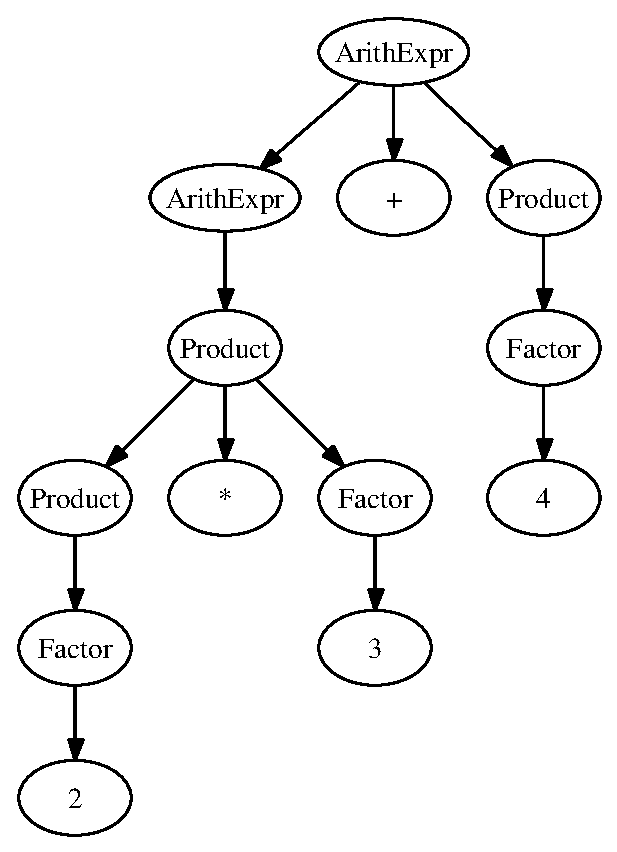
\epsfig{file=Abbildungen/parse-tree.eps, scale=0.6}
  \caption{Ein Parse-Baum f\"ur den String ``\texttt{2*3+4}''.}
  \label{fig:parse-tree.dot2}
\end{figure}

Fassen wir diesen Parse-Baum als Liste seiner
Zweige auf, wobei jeder Zweig eine Liste von Grammatik-Symbolen ist, so erhalten wir die folgende Liste:
\\[0.2cm]
\hspace*{1.3cm}
$
\begin{array}[t]{rl}
  \bigl[ 
 & [ \textsl{ArithExpr}, \textsl{ArithExpr}, \textsl{Product}, \textsl{Product}, \textsl{Factor}, \quoted{2} ],
   \\[0.1cm] 
 & [ \textsl{ArithExpr}, \textsl{ArithExpr}, \textsl{Product}, \quoted{*} ],
   \\[0.1cm] 
 & [ \textsl{ArithExpr}, \textsl{ArithExpr}, \textsl{Product}, \textsl{Factor}, \quoted{3} ],
   \\[0.1cm] 
 & [ \textsl{ArithExpr}, \quoted{+} ],
   \\[0.1cm] 
 & [ \textsl{ArithExpr}, \textsl{Product}, \textsl{Factor}, \quoted{4} ]
   \\[0.1cm] 
  \bigr].
\end{array}
$
\pagebreak

\begin{Definition}[\textsl{parseTree}] \lb
Ist $G = \langle V, T, R, S \rangle$ eine Grammatik, ist $w \in T^*$, $A \in V$ und  gibt es eine Ableitung
\[ A \Rightarrow^* w,  \]
so definieren wir $\textsl{parseTree}(A \Rightarrow^* w)$ induktiv:
\begin{enumerate}
\item Falls $(A \rightarrow t_1t_2 \cdots t_m)\in R$ mit $A \in V$ und $t_i \in T$ f\"ur alle
      $i=1,\cdots,m$, so setzen wir
      \[ \textsl{parseTree}(A \Rightarrow^*t) = \bigl[\, [A, t_1],\,  [A, t_2],\,\cdots,\,  [A, t_m]\, \bigr].  \]
\item Falls  $A \Rightarrow^* w$ gilt, weil
      \[ (A \rightarrow B_1B_2 \cdots B_m) \in R, \quad 
         B_i \Rightarrow^* w_i\; \mbox{f\"ur alle $i=1,\cdots,m$}, \quad
         \mbox{mit} \; w = w_1w_2 \cdots w_m
      \]
      gilt, so definieren wir (unter Benutzung der \textsc{Setl}-Notation f\"ur die Definition von Listen)
      \[ 
        \textsl{parseTree}(A \Rightarrow^*w)  =
        \bigl[\; [A] + l \,:\,
                 i \in [1, \cdots, m ],\, l \in \textsl{parseTree}(B_i \Rightarrow^* w_i) \;
        \bigr]. 
      \]

      Damit diese Definition auch tats\"achlich alle F\"alle abdeckt, m\"ussen wir noch den Fall
      diskutieren, dass  eines der Symbole $B_i$ ein Terminal ist: In diesem Fall setzen wir
      \\[0.2cm]
      \hspace*{1.3cm}
      $\textsl{parseTree}(B_i \Rightarrow^* B_i) := \bigl[ [B_i] \bigr]$.
\end{enumerate}
\end{Definition}

Wir definieren die \emph{Breite} $b$ einer Grammatik als die gr\"o{\ss}te Anzahl von Symbolen, die 
auf der rechten Seite einer Grammatik-Regel der Form
\\[0.2cm]
\hspace*{1.3cm}
$A \rightarrow \alpha$
\\[0.2cm]
auftreten, bei der $\alpha$ kein einzelnes Terminal ist.  Mit dieser Definition ist klar, dass die Breite
einer nicht-trivialen Grammatik in verallgemeinerter Chomsky-Normalform mindestens den Wert zwei hat,
denn eine solche Grammatik enth\"alt ja weder $\varepsilon$-Regeln noch Unit-Regeln.  Falls die Grammatik
also eine Regel enth\"alt, auf deren rechten Seite eine Variable auftritt, dann muss die rechte Seite
dieser Regel mindestens zwei verschiedene Zeichen enthalten.


\begin{Lemma} \label{lemma:length}
  Die Grammatik $G = \langle V, T, R, S \rangle$ habe die Breite $b$.  Ferner gelte
  \\[0.2cm]
  \hspace*{1.3cm}
  $A \Rightarrow^* w$
  \\[0.2cm]
  f\"ur eine syntaktische Variable $A \in V$ und ein Wort $w \in T^*$.  Falls $n$ die L\"ange der l\"angsten Liste in
  \[ \textsl{parseTree}(A \Rightarrow^* w) \]
  ist, so gilt f\"ur die L\"ange des Wortes $w$ die Absch\"atzung
  \\[0.2cm]
  \hspace*{1.3cm}
  $|w| \leq b^{n}$.  
\end{Lemma}

\noindent
\textbf{Beweis}: Wir f\"uhren den Beweis durch Induktion nach  $n$.
\begin{enumerate}
\item[I.A.] $n=2$:  Dann besteht die Ableitung nur aus einem Schritt und daher muss es eine Regel der Form
            \\
            \hspace*{1.3cm}
            $A \rightarrow t_1t_2 \cdots t_m$ \quad mit $w = t_1t_2 \cdots t_m$ und $t_i \in T$
            f\"ur alle $i=1,\cdots,m$
            \\[0.2cm]
            in der Grammatik $G$ geben.  Es gilt dann
            \[ \textsl{parseTree}(A \Rightarrow^* w) = 
               \bigl[\, [A,t_1],\, [A,t_2],\, \cdots,\; [A,t_m]\, \bigr].\, 
            \]
            Daraus folgt
            \\[0.2cm]
            \hspace*{1.3cm}
            $|w| = |t_1t_2 \cdots t_m| = m \leq b \leq b^{2}$,
            \\[0.2cm]
            wobei die Ungleichung $m \leq b$ aus der Tatsache folgt, dass L\"ange der Regeln der Grammatik
            $G$ durch die Breite $b$ beschr\"ankt ist.
\item[I.S.] $n \mapsto n+1$: Da die Ableitung nun aus mehr als einem Schritt besteht, hat die Ableitung die Form
            \\[0.2cm]
            \hspace*{1.3cm}
            $A \Rightarrow B_1 B_2 \cdots B_m \Rightarrow^* w_1 w_2 \cdots w_m = w$.
            \\[0.2cm]
            Au{\ss}erdem haben dann die Listen in
            \[ \textsl{parseTree}(B_i \Rightarrow^* w_i) 
            \]
            f\"ur alle $i=1,\cdots,m$ h\"ochstens die L\"ange $n$.
            Nach Induktions-Voraussetzung wissen wir also, dass
            \\[0.2cm]
            \hspace*{1.3cm}
            $|w_i| \leq b^{n}$ \quad f\"ur alle $i=1,\cdots,m$
            \\[0.2cm]
            gilt.  Daher haben wir
            \\[0.2cm]
            \hspace*{1.3cm}
            $|w| = |w_1| + \cdots + |w_m| \leq b^{n} + \cdots + b^{n} = 
             m \cdot b^n \leq b \cdot b^n \leq b^{n+1}$. \qed
\end{enumerate}

\section{Das Pumping-Lemma f\"ur kontextfreie Sprachen}
\begin{Satz}[Pumping-Lemma]
Es sei $L$ eine kontextfreie Sprache.  Dann gibt es ein $n \in \mathbb{N}$, so dass jeder String
$s \in L$, dessen L\"ange gr\"o{\ss}er oder gleich $n$ ist, in der Form 
\[ s = uvwxy \]
geschrieben werden kann, so dass au{\ss}erdem folgendes gilt:
\begin{enumerate}
\item $|vwx| \leq n$,

      der mittlere Teil des Strings hat also eine L\"ange von h\"ochstens $n$ Buchstaben.
\item $vx \not= \varepsilon$,

      die Teilstrings $v$ und $x$ k\"onnen also nicht beide gleichzeitig leer sein.
\item $\forall h \in \mathbb{N}: uv^hwx^hy \in L$.

      Dieser Bedingung  verdankt das Pumping-Lemma seinen Namen, denn die Strings $v$ und $x$ k\"onnen
      beliebig oft \emph{gepumpt} werden. \qed
\end{enumerate}
\end{Satz}

\noindent
\textbf{Beweis}: Wir zeigen den Satz zun\"achst f\"ur den Fall, dass die Sprache
$L$ das leere Wort nicht enth\"alt.  Dazu konstruieren wir mit dem im letzten Abschnitt gezeigten
Verfahren eine Grammatik $G = \langle V, T, R, S \rangle$ in verallgemeinerter Chomsky-Normalform, so dass
\[ L = L(G) \]
gilt. Wir nehmen an, dass die Grammatik $G$ insgesamt $k$ syntaktische Variablen enth\"alt und au{\ss}erdem die
Breite $b$ hat.  Wir definieren
\[ n := b^{k+2}. \]
Sei nun $s \in L$ mit $|s| \geq n$.  Wir betrachten die Listen aus
\[ \textsl{parseTree}(S \Rightarrow^* s). \]
Falls alle Listen hier eine L\"ange kleiner-gleich $k+1$ h\"atten, so w\"urde aus Lemma
\ref{lemma:length} folgen, dass  
\[ |s| \leq b^{k+1} < n \]
gilt, im Widerspruch zu der Voraussetzung $|s| \geq n$.  Also muss es in 
$\textsl{parseTree}(S \Rightarrow^* s)$ eine Liste geben, die mindestens die L\"ange $k + 2$
hat.  Wir w\"ahlen die l\"angste Liste unter dieser Listen aus.
Diese Liste hat dann die Form
\[ [A_1, \cdots, A_l, t] \quad \mbox{mit $A_i \in V$ f\"ur alle $i \in \{1,\cdots,l\}$},\quad t \in T,
   \quad \mbox{sowie $l \geq k+1$}.
 \]
Wegen $l \geq k + 1$  k\"onnen nicht alle Variablen $A_1$, $\cdots$, $A_l$
voneinander verschieden sein, denn es gibt ja nur insgesamt $k$ verschiedene syntaktische
Variablen.   Wir finden daher in der Menge $\{ l, l-1, \cdots, l-k \}$
zwei Indices $i,j$ mit $i \not=j$ und $A_i = A_j =: A$.  Ohne Beschr\"ankung der Allgemeinheit gelte
$i < j$.   Die Ableitung von $s$ hat dann die folgende Form
\[ S \Rightarrow^* u A_i y \Rightarrow^* u v A_j x y \Rightarrow^* u v w x y = s. \] 
Insbesondere gilt also
\[ S \Rightarrow^* u A y, \quad A \Rightarrow^* vAx, \quad \mbox{und} \quad A \Rightarrow^* w. \]
Damit haben wir dann aber folgendes:
\begin{enumerate}
\item $S \Rightarrow^* uAy \Rightarrow^* uwy$, also
      \[ S \Rightarrow^* uv^0wx^0y. \]
\item $S \Rightarrow^* uAy \Rightarrow^* uvAxy \Rightarrow^* uvvAxxy \Rightarrow^* uvvwxxy$, also
      \[ S \Rightarrow^* uv^2wx^2y. \]
\item $S \Rightarrow^* uAy \Rightarrow^* uvAxy \Rightarrow^* uv^2Ax^2y \Rightarrow^* uv^3Ax^3y
       \Rightarrow^* \cdots \Rightarrow^* uv^kAx^ky \Rightarrow^* uv^kwx^ky$.
\end{enumerate}
Wir m\"ussen jetzt noch zeigen, dass $vx \not= \varepsilon$ gilt.  Die Ableitung
\[ A \Rightarrow^* vAx \]
ist eigentlich die Ableitung
\[ A_i \Rightarrow^* vA_jx \]
und enth\"alt daher mindestens einen Ableitungsschritt.
Wir f\"uhren den Nachweis der Behauptung $vx \not= \varepsilon$ indirekt und nehmen $v = x =
\varepsilon$ an.
Dann w\"urde wegen $A_i = A_j$ also
\\[0.2cm]
\hspace*{1.3cm}
$A_i \Rightarrow^+ A_i$
\\[0.2cm]
gelten. 
Da die Grammatik $G$ nach Voraussetzung keine Unit-Regeln enth\"alt, hat der erste 
Schritt dieser Ableitung dann die Form
\[ A \Rightarrow B_1 B_2 \cdots B_m \Rightarrow^* A \quad \mbox{mit $m \geq 2$}. \] 
Dann muss aber f\"ur wenigstens ein $o \in \{1, \cdots, m\}$
\[ B_o \Rightarrow^* \varepsilon  \]
gelten und das geht nicht, da eine Grammatik in Chomsky-Normalform keine $\varepsilon$-Regeln
enth\"alt.  Also ist die Annahme $vx = \varepsilon$ widerlegt.

Als n\"achstes zeigen wir, dass die Ungleichung $|vwx| \leq n$ gilt.  Wir haben
\[ A = A_i \Rightarrow^* vA_jx \Rightarrow^* vwx. \]
Weil einerseits $i \in \{l-k, l-(k-1), \cdots,l \}$ gilt und andererseits die der
Ableitung
$A \Rightarrow^* vwx$ zugeordnete Liste aus $\textsl{parseTree}(S \Rightarrow^* w)$ von
maximaler L\"ange war, wissen wir, 
dass die L\"ange der l\"angsten Liste in 
\[ \textsl{parseTree}(A \Rightarrow^* vwx) \]
kleiner-gleich  $k+2$ ist.
  Nach dem Lemma
\ref{lemma:length} folgt damit f\"ur die L\"ange von $vwx$ die Absch\"atzung
\[ |vwx| \leq b^{k+2} = n. \]

Zum Schluss m\"ussen wir noch festlegen, was in dem Fall zu tun ist, wenn $\varepsilon \in L$ ist.  
\"Uberf\"uhren wir dann die Grammatik $G$ in verallgemeinerte Chomsky-Normalform, so erhalten wir eine
Grammatik $G'$, f\"ur die
\\[0.2cm]
\hspace*{1.3cm}
$L(G') = L(G) \backslash \{\varepsilon\}$
\\[0.2cm]
gilt.  F\"ur die Sprache $L(G')$ gilt das Pumping-Lemma.  Im Beweis oben haben wir $n = b^{k+2}$
definiert. Damit gilt sicher $n > 0$.  Damit gilt das Pumping-Lemma auch f\"ur das leere Wort, denn
f\"ur das leere Wort $s = \varepsilon$ ist die Voraussetzung $|s| \geq n$
nicht erf\"ullt, so dass die Behauptung des  Pumping-Lemmas f\"ur das leere Wort trivialerweise gilt.
\qed
\vspace*{0.2cm}

\noindent
\textbf{Bemerkung}: Das Pumping-Lemma wird in der deutschsprachigen Literatur gelegentlich auch als 
``\emph{Schleifensatz}'' bezeichnet. 

\section{Anwendungen des Pumping-Lemmas}
Wir zeigen nun, wie mit Hilfe des Pumping-Lemmas der Nachweis erbracht werden kann, dass
bestimmte Sprachen nicht kontextfrei sind.

\subsection{Die Sprache $L = \{ \mathtt{a}^k \mathtt{b}^k \mathtt{c}^k \mid k \in \mathbb{N} \}$ ist
nicht kontextfrei}
Wir weisen nun nach, dass die Sprache
\[ L = \{ \mathtt{a}^k \mathtt{b}^k \mathtt{c}^k \mid k \in \mathbb{N} \} \]
nicht kontextfrei ist.  Wir f\"uhren diesen Nachweis indirekt und nehmen zun\"achst an, dass $L$
kontextfrei ist.  Nach dem Pumping-Lemma gibt es dann eine nat\"urliche Zahl $n$, so dass jeder String
$s \in L$, dessen L\"ange gr\"o{\ss}er oder gleich $n$ ist, sich in Teilstrings der Form
\[ s = uvwxy \]
zerlegen l\"asst, so dass au{\ss}erdem folgendes gilt:
\begin{enumerate}
\item $|vwx| \leq n$,
\item $vx \not= \varepsilon$,
\item $\forall i \in \mathbb{N}: uv^iwx^iy \in L$.

      Insbesondere k\"onnen wir hier $i=0$ w\"ahlen und erhalten dann
      $uwy \in L$. 
\end{enumerate}
Wir definieren nun den String $s$ wie folgt:
\[ s := \mathtt{a}^n\mathtt{b}^n\mathtt{c}^n. \]
Dieser String hat die L\"ange $3 \cdot n \geq n$ und erf\"ullt damit die Voraussetzung \"uber die L\"ange.
Damit finden wir also eine Zerlegung $s=uvwxy$ mit den obigen Eigenschaften.  Da der Teilstring
$vwx$ eine L\"ange kleiner oder gleich $n$ hat, k\"onnen in diesem String nicht gleichzeitig die
Buchstaben \qote{a} und \qote{c} vorkommen. Wir betrachten die nach dieser Erkenntnis noch
m\"oglichen  F\"alle getrennt.
\begin{enumerate}
\item Fall: In dem String $vwx$ kommen nur die Buchstaben \qote{a} und \qote{b} vor,  der Buchstabe
      \qote{c} kommt nicht vor: 
      \\[0.2cm]
      \hspace*{1.3cm}
      $\textsl{count}(vwx,\mathtt{c}) = 0$.
      \\[0.2cm]
      Da $vx \not= \varepsilon$ ist, folgt
      \\[0.2cm]
      \hspace*{1.3cm}
      $\textsl{count}(vx,\mathtt{a}) + \textsl{count}(vx,\mathtt{b}) > 0$.
      \\[0.2cm]
      Wir nehmen zun\"achst an, dass $\textsl{count}(vx,\mathtt{a}) > 0$ gilt,
      der Fall $\textsl{count}(vx,\mathtt{b}) > 0$ ist analog zu behandeln.
      Dann erhalten wir einerseits
      \[ 
      \begin{array}[t]{lcl}
        \textsl{count}(uwy,\mathtt{c}) & = & \textsl{count}(s,\mathtt{c}) - \textsl{count}(vx,\mathtt{c}) \\
                              & = & \textsl{count}(s,\mathtt{c}) - 0 \\
                              & = & \textsl{count}(\mathtt{a}^n\mathtt{b}^n\mathtt{c}^n,\mathtt{c}) \\
                              & = & n.
      \end{array}
      \]
      Z\"ahlen wir nun die H\"aufigkeit, mit welcher der Buchstabe \qote{a}
      in dem String $uwy$ auftritt, so erhalten wir
      \[ 
      \begin{array}[t]{lcl}
        \textsl{count}(uwy,\mathtt{a}) & = & 
        \textsl{count}(s,\mathtt{a})  - \textsl{count}(vx,\mathtt{a}) \\
                              & < & \textsl{count}(s,\mathtt{a}) \\
                              & = & \textsl{count}(\mathtt{a}^n\mathtt{b}^n\mathtt{c}^n,\mathtt{a}) \\
                              & = & n.
      \end{array}
      \]
      Damit haben wir dann aber
      \\[0.2cm]
      \hspace*{1.3cm}
      $\textsl{count}(uwy,\mathtt{a}) < n = \textsl{count}(uwy,\mathtt{c})$
      \\[0.2cm]
      und daraus folgt $uwy \not\in L$, was im Widerspruch zum Pumping-Lemma steht.
\item Fall: In dem String $vwx$ kommt der Buchstabe \qote{a} nicht vor.
   
      Dieser Fall l\"asst sich analog zum ersten Fall behandeln. \qed
\end{enumerate}

\exercise
Zeigen Sie, dass die Sprache 
\[ L = \bigl\{ \,\mathtt{a}^{k^2} \big|\; k \in \mathbb{N}\, \bigr\} \]
nicht kontextfrei ist.
\vspace*{0.2cm}

\noindent
\textbf{Hinweis}: Argumentieren Sie \"uber die L\"ange der betrachteten Strings.

%%% Local Variables: 
%%% mode: latex
%%% TeX-master: "formale-sprachen"
%%% End: 
